\documentclass[14pt,a4paper]{article}
\usepackage[latin1]{inputenc}
\usepackage[T1]{fontenc}
\usepackage[english]{babel}
\usepackage{amsmath}
\usepackage{amsfonts}
\usepackage{amssymb}
\usepackage{makeidx}
\usepackage{amsthm}
\usepackage[margin=48pt]{geometry}
\usepackage[linesnumbered,ruled]{algorithm2e}
\usepackage{tikz}
\usetikzlibrary{automata, positioning}
\usepackage{float}
\usepackage[round]{natbib}
\usepackage[hidelinks]{hyperref}
\usepackage{caption}
\usepackage{graphicx}
\usepackage{subcaption}
%\usepackage[justification=centering]{caption}


\def\code#1{\texttt{#1}}
\newtheorem{theorem}{Theorem}
\def\iff{\Leftrightarrow}
\theoremstyle{definition}
\newtheorem{madef}{Definition}
\newtheorem{prop}{Proposition}


\oddsidemargin  0in
\evensidemargin  0in
\textwidth   6.3in
\textheight  9.5in
\topmargin  -0.7in


\usepackage{fancyhdr}
\pagestyle{fancy}
%\lfoot{Charles DUFOUR}
%\rfoot{\today}
\fancyhead[R]{}


\author{Charles Dufour}
\title{Bachelor Project : \\
Reinforcement learning and robot navigation}
\begin{document}

\begin{titlepage}
\newcommand{\HRule}{\rule{\linewidth}{0.5mm}} % Defines a new command for the horizontal lines, change thickness here

\center % Center everything on the page
 
%----------------------------------------------------------------------------------------
%   HEADING SECTIONS
%----------------------------------------------------------------------------------------

\vspace{3cm}
\textsc{\LARGE \'Ecole polytechnique f\'ed\'erale de Lausanne}\\[0.5cm] % Name of your university/college
\textsc{\large Disopt}\\[1.5cm] % Name of your university/college
\textsc{\LARGE Bachelor project}\\[0.5cm] % Major heading such as course name
\textsc{\large }\\[0.5cm] % Minor heading such as course title

%----------------------------------------------------------------------------------------
%   TITLE SECTION
%----------------------------------------------------------------------------------------

\HRule \\[0.4cm]
{ \huge \bfseries Reinforcement learning and robot navigation}\\[0.4cm] % Title of your document
\HRule \\[1.5cm]
 
%----------------------------------------------------------------------------------------
%   AUTHOR SECTION
%----------------------------------------------------------------------------------------

\begin{minipage}{0.4\textwidth}
\begin{flushleft} \large
\emph{Student:}\\
Charles Dufour
\end{flushleft}
\end{minipage}
~
\begin{minipage}{0.4\textwidth}
\begin{flushright} \large
\emph{Supervisors:} \\
Jonas Racine\\% Supervisor's Name
Prof. Friedrich Eisenbrand 
\end{flushright}
\end{minipage}\\[5cm]

%----------------------------------------------------------------------------------------
%   LOGO SECTION
%----------------------------------------------------------------------------------------

% \includegraphics[width=0.5\linewidth]{Logo}\\[1cm] % Include a department/university logo - this will require the graphicx package
 
%----------------------------------------------------------------------------------------

\vfill % Fill the rest of the page with whitespace

\end{titlepage}



%\begin{titlepage}
%   \vspace*{\stretch{1.0}}
%   \begin{center}
%      \Large\textbf{Reinforcement learning and robot navigation}\\
%      
%      \large\textbf{ }\\
%      \large\textit{Bachelor Project}
%   \end{center}
%   \vspace*{\stretch{2.0}}
%   
%   \vfill 
%   {\centering Charles Dufour, EPFL\par}
%\end{titlepage}

\newpage


\begin{abstract}

This dissertation focuses on the intelligent robot control in autonomous navigation using reinforcement learning. More precisely, the purpose of this bachelor project is to make a robot adapt its behavior based on traffic light using reinforcement learning. Reinforcement learning is a machine learning paradigm in which the agent tries to maximize a numerical reward signal (the reward function) in the long run and has only partial feed-back from the environment (in opposition with supervised learning where the feed-back is complete and unsupervised learning where there is no feed-back) : indeed the agent is not told which action to take but must discover it by trying the actions and see which one yields the best reward.

To make things a little bit more formal, we will introduce Markov Decision Processes (MDP), and then consider model-based and model-free algorithm to solve the problem of learning from partial feedback of the environment. 

Then we will implement on our robot our different algorithm to compare them and then discuss about further work. This project is the successor of many projects on the robot in  DISOPT. 

\nocite{Xia2015}
\nocite{KLMSurvey}
\end{abstract}


\tableofcontents
\pagenumbering{gobble}
\newpage
\fancyhead[L]{\emph{THEORY}}


%\emph{Reinforcement learning}\\
%Reinforcement learning is learning what to do, how to map situations to actions so as to maximize
%a numerical reward signal. The learner is not told which actions to take, but instead must discover
%which actions yield the most reward by trying them. \citep{Sutton}
%
%Some technical terms : 
%\begin{itemize}
%\item \emph{policy} : it is a mapping from the states to the actions
%\item \emph{reward} : what our learning agent is trying to maximize
%\item \emph{model} of the environment : the laws governing the environment 
%\end{itemize}
%
%"Reinforcement learning methods specify how the agent's policy is changed as a result of its experience"\citep{Sutton}
%
%
%
%The usual way to formulate the reinforcement learning problem from a mathematical point of view is by using what we call Markov's decision processes (MDPs).




\pagenumbering{arabic}
\part*{Theory}
\section{Reinforcement learning, a short introduction}

\begin{figure}[H]
\centering
\includegraphics[scale=0.5]{img/RL_graph.png}
\label{RL}
\caption{Graphical representation of the reinforcement learning process from \citep{Sutton}}
\end{figure}

In reinforcement learning problems, a scalar value, which we will call the reward, is received by an agent for transitions to one state to another. The aim of the agent is to maximize the discounted sum of the rewards he will receive, and to do so has to find an appropriate behavior (policy).


Our agent is connected to the model trough perceptions and actions. The typical procedure is as follows: 
\begin{itemize}
\item the environment sends an information to the agent about the state he is actually into
\item then the agent chooses to do an action, based on the information he just received, the action takes him to another state in the environment
\item the environment sends back to the agent a reward (numerical signal) for the transition that just happened and also an information about the state the action brought our agent into
\item and so on $\ldots$
\end{itemize}

The purpose of our agent is to learn an optimal behavior which should optimize the long-run sum of values of the reinforcement signal (the rewards). \citep{KLMSurvey}

We define an \emph{episode} as being a finite sequence of event perceived by our agent (perception,action,reward,\ldots)

\section{MDP : Markov decision processes}



The mathematical way to define the reinforcement learning framework is done using Markov decision processes.

Markov's decision processes are a tuple  $\mathcal{M}=\{\mathcal{S},\mathcal{A},T,R,\gamma\}$ : 

\begin{itemize}
\item a set of states : $\mathcal{S}=\{s_0,s_1,\ldots,s_n\}$
\item a set of actions  : $\mathcal{A}=\{a_1,a_2,\ldots ,a_k\}$
\item a transition function :  $T(s,a,s') \sim  Pr(s'\mid a, s) \quad s,s' \in \mathcal{S}$ which gives the state transition probabilities
\item a reward function : $R:\mathcal{S}\mapsto \mathbb{R} $
\item a discount factor $\gamma \in [0,1)$
\end{itemize}


The discount factor $\gamma $ helps making our learning agent more or less far-sighted : $\gamma$ can be interpreted as the relative importance it will give to future rewards compared to immediate ones.

$\mathcal{M}$ is a MDP if it respects the Markovian property which is that the transitions only depends on the current state and action : 
\begin{equation*}
\mathbb{P}(s_{n+1}\mid a_{n+1},s_{n},a_{n},s_{n-1},\ldots)=\mathbb{P}(s_{n+1}\mid a_{n+1},s_{n})\\
\end{equation*}


When an agent is learning in a MDP, what it observes is a sequence of states, actions and rewards: suppose the agent is in the state $s_0$ and chooses action $a_1$ and then end up in state $s_1$ with reward $r_1$; then the sequence observed is of the form : $s_0,a_1,s_1,r_1,a_2,s_2,r_2\ldots$


Markov decisions processes can easily be  represented as a directed graph : the nodes are the states and the directed edges from a node $Q$ are the actions an agent can choose to make while being in state $Q$, which will bring the agent in the state represented by the node at the endpoint of the edge as we can see in figure \ref{figure : graph_example}.


\begin{figure}[H]
\centering
\captionsetup{justification=centering,margin=2cm}
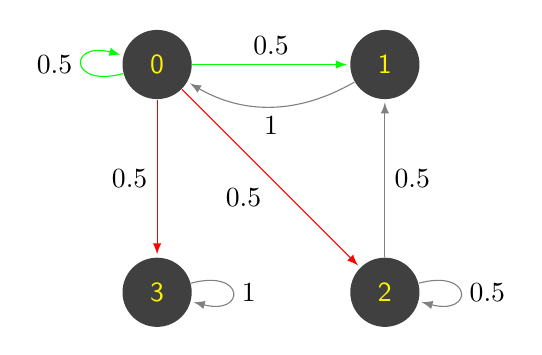
\begin{tikzpicture}[font=\sffamily]
    % Add the states
        \node[state,
              text=yellow,
              draw=none,
              fill=gray!50!black] (0) {0};
        \node[state,
              right=2cm of 0,
              text=yellow,
              draw=none, 
              fill=gray!50!black] (1) {1};
        \node[state,
              below=2cm of 1,
              text=yellow,
              draw=none, 
              fill=gray!50!black] (2) {2};
        \node[state,
        	  below = 2cm of 0,
        	  text=yellow,
        	  draw=none,
        	  fill=gray!50!black] (3) {3};
     

              
 \draw[every loop,
        auto=right,
        >=latex,
        draw=gray,
        fill=gray]
        
        	(0) edge[loop left, draw = green] node {$0.5$}(0)
        	(0) edge[ auto = right,draw = red]  node {$0.5$}(2)
        	(0) edge[auto = right,draw = red] node{$0.5$}  (3)
            (0) edge[auto = left,draw=green]  node {$0.5$} (1)
            (1) edge[bend left,auto =left]  node {$1$} (0)
            (2) edge[]  node {$0.5$}(1)
			(2) edge[loop right] node{$0.5$} (2)
			(3) edge[loop right] node{$1$} (3)	
			       
            ;       
      
    \end{tikzpicture}
    \label{figure : graph_example}
    \caption{example of a graph representing a Markov Decision process, there are two actions possible from node $0$ which takes to different states with some probability }
     \label{figure : graph_example}
   
\end{figure}  




\section{Policies and Value functions}

A policy : $\pi $ is a stochastic mapping from states to action: $$ \pi : \mathcal{A} \times \mathcal{S} \mapsto [0,1] \quad \text{s.t. } \sum_{a}\pi(a\mid s)=1 \quad \forall s \in \mathcal{S}$$
A policy is a formalisation of the decision making process : in each state, we follow the policy to decide which action to choose with some probability: $\pi(a\mid s) $ is the probability that $A_{t+1}=a$ if $S_t=s$.Hence maximizing the reward means finding a good policy.


We need to quantify the reward the agent has to maximize, so we define the return as : 
$$G_t= r_{t+1}+\gamma r_{t+2}+ \dots = \sum_{k=0}^{\infty}\gamma^{k}r_{t+k+1} = r_{t+1} + \gamma G_{t+1} $$





Now we need a way to compare policy between them : for that we use the \emph{value functions} : the state value and the state-action value under a certain policy $\pi$. Intuitively they measure how good it is to be in a state (or respectively to take a specific action while being in a state) if we follow the policy afterwards.


Then we can define the value of taking action $a$ in state $s$ while following the policy $\pi$ as the expected return we would receive if we follow $\pi$:


\begin{equation*}
\begin{split}
v_{\pi}(s)&= \mathbb{E}_{\pi}[G_t \mid S_t=s]
\\&=\mathbb{E}_{\pi}\left[ r_{t+1} + \gamma G_{t+1} \mid S_t = s\right]
\\&=\mathbb{E}_{\pi}\left[ r_{t+1} \mid S_t = s \right] + \gamma \mathbb{E}_{\pi}\left[G_{t+1} \mid S_t = s \right]
\\&=\sum_{a}\pi(a \mid s)\sum_{s'}\mathbb{P}(s' \mid a,s)R(s') 
\\&+ \gamma \sum_{a}\pi(a \mid s)\sum_{s'}\mathbb{P}(s'\mid a,s)\mathbb{E}_{\pi}\left[G_{t+1} \mid S_{t+1} = s', S_{t}= s\right]
\end{split}
\end{equation*}

Using the Markovian property, $\mathbb{E}_{\pi}\left[G_{t+1} \mid S_{t+1}, S_{t}\right] = \mathbb{E}_{\pi}\left[G_{t+1} \mid S_{t+1}\right] $ so we get : 

\begin{equation}
\begin{split}
v_{\pi}(s)&= \sum_{a}\pi(a \mid s)\sum_{s'}\mathbb{P}(s'\mid a,s)\left[R(s') +\gamma \mathbb{E}_{\pi}\left[  G_{t+1} \mid S_{t+1}=s'  \right]\right]
\\&=\sum_{a}\pi(a \mid s)\sum_{s'}\mathbb{P}(s'\mid a,s)\left[R(s') + \gamma v_{\pi}(s')\right]
\end{split}
\label{v(s)}
\end{equation}



And the value of taking action $a$ while being in state $s$ under a policy $\pi$ following roughly the same method:

\begin{equation}
\begin{split}
q_{\pi}(s,a)&= \mathbb{E}\left[G_t\mid S_t=s, A_t=a\right]
\\&=\mathbb{E}\left[\sum_{k=0}^{\infty}\gamma^{k}r_{t+k+1}\mid S_t=s,A_t=a\right]
\\&= \sum_{s'}\mathbb{P}(s'\mid a,s)\left[R(s')+\gamma v_{\pi}(s')\right]
\end{split}
\label{q(s,a)}
\end{equation}



We can see from equations (\ref{v(s)}) and (\ref{q(s,a)})  that : 
\begin{equation}
v_{\pi}(s)=\sum_{a}\pi(a\mid s)q_{\pi}(s,a)
\end{equation}

These equations are called the Bellman equations and are used to find the value functions using dynamic programming, since they give recursive definition of the value functions.




\section{Optimal policies and Optimal value function}

For finite MDPs, the value function can define a partial order in the space of policies : 
$$ 
\pi\leq \pi' \iff v_{\pi} (s)\leq v_{\pi'} (s) \quad \forall s \in \mathcal{S}
$$

An optimal policy is a policy which is greater or equal than any other policy. This is what we are interested to find.

We can notice there is no policy strictly better than every deterministic policy \citep{Puterman} so there is always a deterministic optimal policy since there is only a finite number of deterministic policies.


We may have multiple optimal policies but they all have the same value functions otherwise they would not be optimal policies with respect to the partial order define earlier. We denote these functions $q_{*}$ and $v_{*}$.

\paragraph{Bellman optimality equations}

The optimal policy $\pi^*$ has  optimal value functions : $v_* $ and $ q_*$, which satisfy the relations below : 

\begin{equation}
\begin{split}
v_{*}(s)&=\max_{a}q_{*}(s,a)
\\&=\max_{a} \sum_{s'}\mathbb{P}(s'\mid a,s)\left[R(s')+\gamma v_{*}(s')\right]
\end{split}
\label{bellman_opt_v}
\end{equation}

\begin{equation}
\begin{split}
q_{*}(s,a)&=\mathbb{E}\left[ R_{t+1} + \gamma v_{*}(S_ {t+1}) \mid S_t = s, A_t = a \right]
\\&=\mathbb{E}\left[ R_{t+1} + \gamma \max_{a'} q_{*}(S_{t+1},a') \mid S_t = s, A_t = a \right]
\\&= \sum_{s'}\mathbb{P}(s' \mid s,a)[R(s')+\gamma \max_{a'}q_{*}(s',a')]
\end{split}
\label{bellman_opt_q}
\end{equation}

These are called the \emph{Bellman optimality equations}. What equation (\ref{bellman_opt_v}) tells intuitively is that the value of a state under $\pi^*$ must equal the expected return for the best action we can take from that state.


For finite MDPs these equations have a unique solution. We can note that if we know $v_{*}$ or $q_{*}$ a greedy approach to define a policy (best in the short term) becomes a long-term optimal solution : indeed defining a policy being greedy in function of $v_*$ implies that you go to the best state possible, the one with the biggest expected reward.


\section{Solving MDPs with dynamic programming}

In general we don't have all the information we need to compute the exact value of $v_{*}$ or even if we have them, we don't have the computational 
power needed. We often use approximation of value-function instead.


From now on we assume our MDPs are finite, even if it is possible to extend everything to infinite MDPs if we are careful enough to avoid the problematic ones. \citep{Sutton}

\subsection{Policy iteration}

This method uses two processes : the first one is policy evaluation : we compute the value function of a policy for all the states $s \in \mathcal{S} $; then we use policy improvement to get a better policy by acting greedy.
\paragraph{Policy evaluation} 


We begin by setting arbitrary $v(s) \quad \forall s \in \mathcal{S}$.
Then we update using one of the following update rules : 

\begin{itemize}
\item $v_{k+1}(s)=\underset{a \in A}{\sum}\pi(a \mid s)\underset{s'}{\sum}\mathbb{P}(s'\mid a,s)(R(s')+\gamma v_k(s'))$ \quad this is called "iterative policy evaluation".
\item we can use the same update rule as before, but use new information as soon as it is available : this kind of upgrade algorithm are called in places.
\end{itemize}

From this we derive the algorithm \ref{algo1}.


\begin{algorithm}
\label{algo1}
    \SetKwInOut{Input}{Input}
    \SetKwInOut{Output}{Output}

    %\underline{function Euclid} $(a,b)$\;
    \Input{policy to evaluate $\pi$}
    \Output{$V \approx v_{\pi}$}
    Initialize $V = 0$\\
    \While{$\Delta \geq \epsilon$}{
    	$\Delta = 0$\\
    	\For{$s\in \mathcal{S}$}{
    	 $v=V(s)$\\
    	 $V(s)=\underset{a}{\sum}\pi(a\mid s)\underset{s'}{\sum}\mathbb{P}(s'\mid a,s)[R(s')+\gamma V(s')]$\\
    	 $\Delta = \max(\Delta,\mid v-V(s)\mid)$\\
    	 }
       	}
       	\Return{$V \approx v_{\pi}$}
    
    \caption{Iterative policy evaluation (in place)}
\end{algorithm}





\paragraph{Policy improvement}

Then we try to find a better policy : we try to determine whether we should change $\pi(s) $ to $ a\neq\pi(s)$. In order to do so, we try to first select action $a$ while being in state $s$ and then following the policy. If the expected reward we get by doing this choice is better than the one we get by simply following our policy, we should improve.

Mathematically speaking we will compare the value of taking action $a$ while being in the state s : $q_{\pi}(s,a)$ to the value of $s$: $v_{\pi}(s)$. Then we would greedily improve our policy this way.

The greedy update rule we use to improve our policy is the idea behind algorithm \ref{algo2} : 

$$ 
\pi'(s)=\text{arg}\max_{a \in A}q_{\pi}(s,a)
$$

\begin{algorithm}
\label{algo2}
    \SetKwInOut{Input}{Input}
    \SetKwInOut{Output}{Output}

    %\underline{function Euclid} $(a,b)$\;
    \Input{policy to improve $\pi$}
    \Output{$\pi'$ s.t : $\pi' \geq \pi$ }
    \For{$s\in \mathcal{S}$}{
    	$\pi'(s)=\underset{a \in A}{\text{argmax }}q_{\pi}(s,a)$
    	}
       	\Return{$\pi'$}
    
    \caption{Policy improvement}
\end{algorithm}



\paragraph{Policy Iteration} By combining the two processes described before, we can derive an algorithm to sweep through all our states and upgrade our policy until the changes between each sweep is too small : it is controlled by a parameter $\epsilon$ and a parameter $\gamma$ (which we talked about previously).This is the algorithm \ref{algo3} which can be represented graphically by figure (\ref{fig:Sutton})



\begin{figure}[ht]
\centering
\includegraphics[scale=0.7]{img/policy_iter_sutton.PNG}
\caption{Graphical representation of the interactions between policy improvement and policy evaluation(from \citep{Sutton})}
\label{fig:Sutton}
\end{figure}






Algorithm \ref{algo3} terminates since there is only a finite number of deterministic policies.
The reason why the algorithm~\ref{algo3} works is called the the \emph{policy improvement theorem}:

\begin{theorem}
Let $\pi$ and $\pi'$ be any pair of policies such that  $\forall s \in \mathcal{S} : $
\begin{equation}
q_{\pi}(s,\pi(s))\geq v_{\pi'}(s) \label{th1}
\end{equation}
then :
\begin{equation}
\pi \geq \pi' \label{th2}
\end{equation}


Moreover if there is a strict inequality in all the states in \ref{th1} then there must be at least a strict inequality for one state in \ref{th2}
\end{theorem}


\begin{proof}
The idea of the proof is to expand the $q_{\pi}$ side until we get $v_{\pi'}(s)$ using Equation~\ref{q(s,a)} in page \pageref{q(s,a)}.

Indeed we have : 
\begin{equation}
\begin{split}
v_{\pi}(s) &\leq q_{\pi}(s,\pi'(s))
\\&=\mathbb{E}[r_{t+1}+\gamma v_{\pi}(S_{t+1})\mid S_{t}=s, A_{t}=\pi'(a)]
\\&=\mathbb{E}_{\pi'}[r_{t+1}+\gamma v_{\pi}(S_{t+1})\mid S_{t}=s]
\\& \leq \mathbb{E}_{\pi'}[r_{t+1}+\gamma q_{\pi}(S_{t+1},\pi'(S_{t+1}) \mid S_{t}=s]
\\& = \mathbb{E}_{\pi'}[r_{t+1}+\gamma \mathbb{E}_{\pi'}[r_{t+2}+\gamma v_{\pi}(S_{t+2})]\mid S_{t}=s]
\\& = \mathbb{E}_{\pi'}[r_{t+1}+\gamma r_{t+2}+\gamma^2 v_{\pi}(S_{t+2})\mid S_{t}=s]
\\& \leq \ldots
\\&= v_{\pi'}(s)
\end{split}
\end{equation}
\end{proof}


\begin{algorithm}
	\SetKwInOut{Input}{Input}
    \SetKwInOut{Output}{Output}
    
	\Input{arbitrary policy, stopping criterion $\epsilon$}
	\Output{estimation of the optimal policy and of its value function}
	
	Policy evaluation :\\
	    \While{$\Delta \geq \epsilon$}{
    	$\Delta = 0$\\
    	\For{$s\in \mathcal{S}$}{
    	 $v=V(s)$\\
    	 $V(s)=\underset{a}{\sum}\pi(a\mid s)\underset{s'}{\sum}\mathbb{P}(s'\mid a,s)[R(s')+\gamma V(s')]$\\
    	 $\Delta = \max(\Delta,\mid v-V(s)\mid)$\\
    	 }
       	}
     
     Policy improvement : \\
     policy-stable = true \\
     \For{$s \in \mathcal{S}$}{
     old-action= $\pi(s)$\\     
     $\pi(s)=\underset{a \in A}{\text{argmax}}q_{\pi}(s,a)$\\
     \If{old-action $\neq \pi(s)$}{
     policy-stable = false}
     }
     \eIf{policy-stable}{
     \Return{$V \approx v^{*} \text{and} \quad \pi \approx \pi^{*}$}
     }{Go to Policy evaluation}
     
	\caption{Policy Iteration}
	\label{algo3}
\end{algorithm}







\subsection{Other types of DP method}

\paragraph{Value Iteration}
Value iteration is another way of approximating an optimal policy : it combines in each of its sweep improvement and evaluation in algorithm \ref{algo4}.

\begin{algorithm}[H]
	\SetKwInOut{Input}{Input}
    \SetKwInOut{Output}{Output}
    \label{algo4}
    
    \Input{policy}
    \Output{estimate of optimal policy}    
	    
    Initialize V arbitrarily 
    \While{$\Delta \geq \epsilon$}{
    	$v=V(s)$\\
    	$V(s)=\underset{a}{\max}\underset{s'}{\sum}\mathbb{P}(s'\mid s,a)[R(s')+\gamma v_{k}(s')]$\\
    	$\Delta =\max(\Delta,\mid v-V(s) \mid)$\\    	
    }
    \Return{$\pi \approx \pi^{*}$ s.t : $\pi(s)=\underset{a}{\text{argmax}}\underset{s'}{\sum}\mathbb{P}(s'\mid s,a)[R(s')+\gamma v_{k}(s')]$}
    

    
\caption{Value iteration}
\end{algorithm}



Algorithm \ref{algo4} finishes if the number of states is finite : 
\begin{proof} 
We define the Bellman operator : $\mathcal{T}:\mathbb{R}^{\mid \mathcal{S}\mid } \mapsto \mathbb{R}^{\mid \mathcal{S}\mid }$ in the following way :
\begin{equation*}
(\mathcal{T}V)(s)=\max_{a \in \mathcal{A}}\sum_{s'}\mathbb{P}(s'\mid a,s)\left[ R(s') + \gamma V(s') \right]
\end{equation*}

In particular this operator is a contraction in the infinity norm, and hence our convergence is equivalent to the well known fixed point problem. Indeed if we consider the inequality : 
\begin{equation}
\mid \max_{z}f(z)-\max{z}h(z)\mid \leq \max_{z}\mid f(z) - h(z)\mid
\label{inter}
\end{equation}
Then having this inequality:
\begin{equation*}
\begin{split}
\mid \mathcal{T}V(s) - \mathcal{T}V'(s) \mid & \leq \mid \max_{a \in \mathcal{A}}\sum_{s'}\mathbb{P}(s'\mid a,s)\left[ R(s') + \gamma V(s') \right] - \max_{a \in \mathcal{A}}\sum_{s'}\mathbb{P}(s'\mid a,s)\left[ R(s') + \gamma V'(s') \right]\mid
\\& \stackrel{(\ref{inter})}{\leq} \max_{a \in \mathcal{A}}\mid \sum_{s'}\mathbb{P}(s'\mid a,s)\left[ R(s') + \gamma V(s') \right] - \sum_{s'}\mathbb{P}(s'\mid a,s)\left[ R(s') + \gamma V'(s') \right]\mid
\\&\leq \max _{a}\gamma \mid \sum_{s'}\mathbb{P}(s'\mid a,s)\left[ V(s')-V'(s')\right] \mid
\\& \leq \gamma \max_{s} \mid V(s)-V'(s) \mid
\\& \leq \gamma \mid \mid V-V'\mid \mid _{\infty}
\end{split}
\end{equation*}

Now using the property that a contraction has a unique fixed point and that all sequences $V,\mathcal{T}V,\mathcal{T}^2V,\ldots $ converges towards this fixed point we get the convergence.


\end{proof}





There exists some others dynamic programming algorithm to solve these problems : 
\begin{itemize}
\item Asynchronous Dynamic programming : it doe not sweep amongst all the states at each iteration. They are in place iterative DP algorithms.
\item General Policy Iteration (GPI): they are mixing the two components of policy iteration (evaluation and improvement) a little bit more than the algorithm we already saw.
\end{itemize}

But the most important drawback to these methods is that they are model-based, meaning that we need to have a complete knowledge of the model to implement those.

\section{model-free approaches and algorithms}

Until now, we assumed implicitly that we knew the model (i.e. the transition function) of our environment all the previous learning algorithm where based on this assumption. Hence we call them \emph{model based}, meaning that you can not apply them if you do not know the model. But in real life applications, we often do not know the whole model, and we have to study other methods in order to do reinforcement learning : this is what gives us the \emph{model free} algorithms. We will discuss shortly some of them in this section.

\subsection{Monte-Carlo methods}
Monte-Carlo methods use sampling from episodes to estimate the action value function.
They differ from the dynamic programming methods by the fact that they do not require a knowledge of the model to estimate the action value function of a policy. To improve our policy, we still use the same greedy approach as before, choosing the best actions available in each state.
Monte-Carlo methods estimate the value function by averaging the sample return from the episodes. Thus they only need sample sequences of state, action, reward from experience or simulation. \citep{Sutton}


 It can be shown to converge as long as all pairs $(s,a)$ with $s$ a state, and $a$ an action are visited an infinite number of time.
\subsection{Temporal difference methods}
Temporal difference methods are a combination of dynamic programming and Monte-Carlo methods : unlike Monte Carlo methods, TD learning methods do not have to wait until an estimate of the return is available (i.e., at the end of an episode) to update the value function. Instead, they use temporal errors and only have to wait until the next time step. The temporal error is the difference between the old estimate and a new estimate of
the value function, taking into account the reward received in the current sample.
These updates are done iteratively and, in contrast to dynamic programming
methods, only take into account the sampled successor states. \citep{Xia2015}

\paragraph{Q-learning} Estimation of the optimal action value function $q_*$:


with $s'$ the state resulting from action a :
\begin{equation}
Q(s,a) \leftarrow Q(s,a) + \alpha \left( \mathcal{R}(s') + \gamma \max_{a'}Q(s',a') - Q(s,a) \right) 
\label{eq:ql}
\end{equation}

Where $\alpha$ is the learning factor.

\begin{proof} (convergence of Q-learning algorithm)
See \citep{Watkins_article}
\end{proof}


\paragraph{SARSA} Estimation of the action value function $q_{\pi}$:

with the action $a'$ being chosen following the policy $\pi$:
\begin{equation}
Q(s,a) \leftarrow Q(s,a) + \alpha \left( \mathcal{R}(s') + \gamma Q(s',a') - Q(s,a) \right)
\end{equation}



\newpage
\part*{Implementation}
\fancyhead[L]{\emph{IMPLEMENTATION}}
We have to determine our states, and hence a way for the robot to find its relative distance to our traffic light.
\section{The robot}
The robot is a raspberry pi 3 powered robot with a camera, like in Figure (\ref{fig:sub1}).

\begin{figure}[H]
\centering
\begin{subfigure}{.5\textwidth}
  \centering
  \includegraphics[width=.5\linewidth]{img/robot.png}
  \caption{The raspberry pi 3 powered robot with one camera}
  \label{fig:sub1}
\end{subfigure}%
\begin{subfigure}{.5\textwidth}
  \centering
  \includegraphics[width=.5\linewidth]{img/setting1_mod1.png}
  \caption{The setting}
  \label{fig:sub2}
\end{subfigure}
\caption{The Framework of our runs}
\label{fig:test}
\end{figure}



\section{The task}
The robot can already follow lines from previous projects on it, and we want to learn how to respect a traffic light using reinforcement learning. 

\section{Modelization}

\subsection{States}
The states are modeled in the following way : in one state we have to have the information about the distance to the traffic light if there is one, the color of the traffic light and the actual speed of the robot.

One can represent the states in the following way : we have a graph like the one in Figure  (\ref{figure : graph_example}) for each speed, for example in Figure~(\ref{figure : graph_ex}). Then we add as a second layer the information about the traffic light color.
\begin{figure}[H]
\begin{center}
    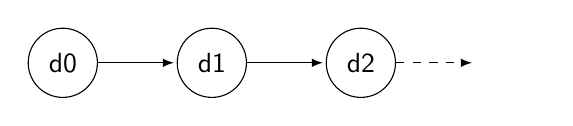
\begin{tikzpicture}[font=\sffamily]
    % Add the states
        \node[state,text=black] (d0) {d0};    
        \node[state,right = 1cm of d0,text=black] (d1) {d1};
        \node[state,right = 1cm of d1,text=black] (d2) {d2};
        \node[state,right = 1cm of d2,text=black,draw=none] (d3) {};       
              
        % Connect the states with arrows
        \draw[every loop,auto=right,>=latex,draw=black,fill=black]
        	(d0) edge[] (d1)
        	(d1) edge[] (d2)
        	(d2) edge[dashed] (d3)
            ;
    \end{tikzpicture}
\end{center}
    \caption{Exemple of a transition graph for a certain speed}
    \label{figure : graph_ex}

\end{figure}


The robot can go from speed $20$ to spedd $100$  and we decided to consider the speeds $20,25,30,25,\ldots$ for simplicity.

The distance to the traffic light is computed in the following way. The traffic light is actually a phone, which accesses the website \url{http://light.grathink.com}. The robot perceives images as the image~(\ref{vue_robot}) and the algorithm for the image processing is algo (\ref{detection_image}).

\begin{figure}
\centering
\captionsetup{justification=centering,margin=2cm}
\includegraphics[scale=0.7]{img/vue10.png}
\caption{View from the robot's camera in our setting (the image is seen like this, rotating it would be computationally costly); in green is the point from where the distance is computed, the lines are the area of the search of the robot and in yellow are the point use to detect the presence of the traffic light}
\label{vue_robot}
\end{figure}



\begin{algorithm}
	\SetKwInOut{Input}{Input}
    \SetKwInOut{Output}{Output}
    
	\Input{an image from the camera feed of the robot}
	\Output{distance, color of the traffic light}
	
	Scan the searching area for bright white pixels\\
	Find the middle of the zone of the white pixels\\
    From there go down to the bottom of the traffic light (end is detected as a value in all the RGB channel big enough)\\
    distance = the number of pixels from the top of the image to the bottom of the traffic light\\
    color is determined from the intensity of the different RGB channel
	\caption{Image processing}
	\label{detection_image}
\end{algorithm}

Now our robot has a way to perceives in which state he is. What action can he take ? 


\subsection{Actions}
The action we are interested in do not concern the direction, which is imposed from the line on the ground as we can see from Figure (\ref{fig:sub2}). Hence we are only interested in accelerating or slowing down. The possible actions are to go from one speed to any other speed (can be easily done through the already coded functions on the robot).
\subsection{Reward function}

\section{Simulation of the model}

One can apply Q-learning on a modelization of the problem : we do not have to have the robot running around into walls and whatever to learn; if we can have a modelization of our problem, we could run everything in a simulated world and after that actually transfer the results to the robot directly.
\section{Results}
















\nocite{Watkins_phd}
\newpage
\fancyhead[L]{\emph{BIBLIOGRAPHY}}


\bibliographystyle{apa-good}
\bibliography{ref}
\addcontentsline{toc}{section}{References}


\end{document}
